% Глава 4. Материал: docs/architecture/, docs/adr/, docs/data/, docs/security/, docs/pedagogy/,
% docs/process/agent-harness.md, src/muallim/. Рисунки: fig-context, fig-layers, fig-pipeline, fig-harness,
% экраны figures/screen-card.png, figures/screen-result.png (снимки docs/design/screens/ на 2026-10-18).
\chapter{Реализация}\label{ch:impl}

Глава описывает оба артефакта в версии 0.6.0. Разделы~\ref{sec:impl-overview}--\ref{sec:impl-privacy}
посвящены тренажёру: контексту, программе, архитектуре, конвейеру оценки, интерфейсу ученика,
исследовательским данным и приватности. Раздел~\ref{sec:impl-harness} описывает обвязку разработки,
раздел~\ref{sec:impl-verification} --- проверку обоих.

\section{Обзор}\label{sec:impl-overview}

Рисунок~\ref{fig:context} показывает систему в её окружении. Ученик общается с тренажёром через Telegram
Bot API кнопками и голосовыми сообщениями. Тренажёр берёт уроки из программы, собранной по книге,
отправляет аудио ученика распознавателю Quran Muaalem и сохраняет попытки, ошибки и разметку в
PostgreSQL; аудиофайлы хранятся отдельно и только с согласия. Исследователь работает с данными через
утилиту командной строки, которая строит отчёты, готовит пакеты разметки и выгружает наборы данных.
Разметчики --- два преподавателя --- размечают попытки в Telegram или в табличных пакетах.

\begin{figure}[ht]
\centering
\resizebox{0.95\linewidth}{!}{% Контекст системы (C4, уровень 1). Источник смысла: docs/architecture/diagrams/01-context.mmd.
\begin{tikzpicture}[node distance=6mm and 9mm]
  \node[human,text width=2.6cm] (learner) {\LANG{Learner}{Ученик}\\[-1pt]{\scriptsize\LANG{Russian-speaking beginner}{русскоязычный новичок}}};
  \node[box,right=of learner,text width=2.2cm] (tg) {Telegram\\Bot API};
  \node[hot,right=of tg,text width=3.0cm] (bot) {\LANG{Tutor bot}{Бот-тренажёр}\\[-1pt]{\scriptsize Python 3.12, aiogram 3}};
  \node[box,above=of bot,text width=3.0cm] (book) {\LANG{Curriculum}{Программа}\\[-1pt]{\scriptsize\LANG{125 lessons, book order}{125 уроков в порядке книги}}};
  \node[box,right=of bot,text width=2.6cm] (model) {Quran Muaalem\\[-1pt]{\scriptsize\LANG{phoneme recogniser}{распознавание фонем}}};
  \node[store,below=of bot,text width=2.9cm,minimum height=1.1cm] (db) {PostgreSQL\\[-1pt]{\scriptsize\LANG{attempts, errors, labels}{попытки, ошибки, метки}}};
  \node[store,right=of db,text width=2.4cm,minimum height=1.1cm] (audio) {\LANG{Audio store}{Записи}\\[-1pt]{\scriptsize\LANG{consent only}{только с согласия}}};
  \node[box,left=of db,text width=2.9cm] (cli) {muallim-research\\[-1pt]{\scriptsize\LANG{reports, labels, dataset}{отчёты, разметка, датасет}}};
  \node[human,below=of cli,text width=2.6cm] (res) {\LANG{Researcher}{Исследователь}};
  \node[human,below=of db,text width=2.9cm] (ann) {\LANG{Annotators}{Разметчики}\\[-1pt]{\scriptsize\LANG{two teachers}{два преподавателя}}};

  \draw[arr] (learner) -- node[lab,below]{\LANG{voice, taps}{голос, кнопки}} (tg);
  \draw[arr] (tg) -- (bot);
  \draw[arr] (book) -- (bot);
  \draw[arr] (bot) -- (model);
  \draw[arr] (bot) -- (db);
  \draw[arr] (bot.south east) -- (audio.north west);
  \draw[arr] (res) -- (cli);
  \draw[arr] (cli) -- (db);
  \draw[arr,<->] (ann) -- node[lab,left,pos=0.3]{\LANG{labels}{метки}} (db);
  \begin{scope}[on background layer]
    \node[group,fit=(bot)(book)(db)(audio)(cli)(model),label={[lab,anchor=south east]north east:\LANG{system boundary}{граница системы}}] {};
  \end{scope}
\end{tikzpicture}
}
\caption{Контекст системы (Р-01).}\label{fig:context}
\end{figure}

Код написан на Python 3.12, около 9\,000 строк в 92 модулях. Основные технологии и причины выбора --- в
таблице~\ref{tab:stack}.

\begin{table}[ht]
\centering\small
\caption{Технологии.}
\label{tab:stack}
\begin{tabularx}{\linewidth}{@{}P{3.2cm}P{4.2cm}L@{}}
\toprule
Задача & Выбор & Причина \\
\midrule
Мессенджер & Telegram, aiogram 3 & Аудитория уже им пользуется; голосовые; асинхронная типизированная
библиотека. \\
Распознаватель & Quran Muaalem \cite{SRC-003} & Открытый, на уровне фонем, с артикуляционными
признаками. \\
Внедрение зависимостей & dishka \cite{SRC-008} & Области приложения и запроса; интеграция с aiogram. \\
База данных & PostgreSQL 16, SQLAlchemy Core, Alembic & Исследовательские данные с миграциями; SQLite в
тестах. \\
Проверка архитектуры & import-linter \cite{SRC-009} & Контракты слоёв в CI и в стоп-хуке агента. \\
Качество & pytest, Hypothesis, mypy --strict, ruff & Быстрые тесты без модели и сети; строгие типы. \\
Сборка & uv, Docker & Lock-файл; воспроизводимый образ; модель как необязательное дополнение. \\
\bottomrule
\end{tabularx}
\end{table}

\section{Программа по книге}\label{sec:impl-curriculum}

\paragraph{Издание и расшифровка} Выбрано альметьевское издание 2010~г. \cite{SRC-040}: это полное
современное издание духовного управления в орфографии Мединского мусхафа --- той же, что в данных модели,
--- а его порядок букв совпадает с независимым узбекским изданием, что указывает на порядок самого Максуди.
Страницы с упражнениями 10--85 расшифрованы построчно. Скан книги хранится локально, вне системы контроля
версий и вне бота: издание защищено авторским правом, поэтому в тренажёре только арабские упражнения и
собственные объяснения, без русского текста книги.

\paragraph{От страниц к урокам} Урок соответствует разделу книги; длинные разделы делятся на части не
длиннее восьми строк. Карточка соответствует напечатанной строке и хранит номер страницы и строки, так что
любую попытку можно проследить до книги. Результат --- в таблице~\ref{tab:book}: вся книга в девяти
частях, 125 уроков и 800 карточек.

\begin{table}[ht]
\centering\small
\caption{Книга как учебная программа.}
\label{tab:book}
\begin{tabular}{@{}lrrr@{}}
\toprule
Часть & Уроков & Карточек & Страницы \\
\midrule
1. Знакомство (\emph{истиаза}, \emph{басмала}, алфавит) & 2 & 8 & 10 \\
2. Буквы и краткие гласные & 28 & 128 & 10--24 \\
3. Долгие гласные & 7 & 50 & 25--29 \\
4. \emph{Шадда} и \emph{танвин} & 7 & 52 & 30--34 \\
5. Хамза, артикль, \emph{сукун} & 9 & 62 & 35--42 \\
6. \emph{Мим} и \emph{нун} & 17 & 116 & 43--54 \\
7. Особенности письма Корана & 15 & 113 & 55--62 \\
8. Остановка и \emph{мадд} & 11 & 78 & 63--74 \\
9. Суры & 29 & 193 & 75--85 \\
\midrule
Всего & 125 & 800 & 10--85 \\
\bottomrule
\end{tabular}
\end{table}

\paragraph{Строение урока} Урок буквы начинается с короткой карточки-правила простым русским языком («как
произносить»), затем даёт букву с \emph{фатхой}, \emph{кясрой} и \emph{даммой} тремя отдельными карточками, а
затем --- строки книги. Строки, отмеченные в книге «обратите внимание», где противопоставлены похожие
звуки, помечены как минимальные пары. Экран «Знаки» объясняет огласовки и другие значки до того, как они
понадобятся.

\paragraph{Примеры из Корана} Начиная со с.~38 книга цитирует Коран. Вместо переноса огласовок со скана
каждая из 139 коранических строк сопоставлена с текстом Мединского мусхафа по скелету согласных и взята из
мусхафа со ссылкой «сура:аят» \cite{SRC-041}; две строки без совпадения расшифрованы со скана. Это снижает
число ошибок в самой чувствительной части контента.

\paragraph{Версии и сверка} Программа хранится в YAML, который собирается скриптом из расшифровки. Каждая
версия публикуется в базу данных как снимок, поэтому каждая попытка указывает на тот текст, который видел
ученик, даже если программа позже изменится; бот не запускается, если контент изменён без новой версии.
Строки, расшифрованные со скана, помечены \texttt{verified: false}, пока автор не сверит их со сканом;
изменение контента --- зона только человека.

\section{Архитектура}\label{sec:impl-architecture}

\subsection{Слои}

Код организован слоями с фиксированным направлением зависимостей (рис.~\ref{fig:layers}). Доменный слой
содержит правила оценки, типы ошибок, модель программы и политику оценки и использует только стандартную
библиотеку Python. Прикладной слой содержит сценарии и \emph{порты} --- интерфейсы, через которые сценарии
обращаются к внешнему миру: распознаватель, репозитории, хранилище аудио, подсказка чтения. Слой
инфраструктуры реализует порты через PostgreSQL, Muaalem, ffmpeg и YAML; слой представления содержит
обработчики и экраны Telegram; исследовательский слой строит отчёты и выгрузки; слой запуска хранит
конфигурацию, контейнер зависимостей и точки входа. Пять контрактов import-linter обеспечивают эти
правила --- например, что домен ничего не импортирует, а представление никогда не импортирует
инфраструктуру.

\begin{figure}[ht]
\centering
\resizebox{0.9\linewidth}{!}{% Слои и разрешённые зависимости (ADR-0002); нарушение ловит import-linter.
\begin{tikzpicture}[node distance=4.5mm and 6mm, every node/.style={font=\sffamily\small}]
  \node[soft,text width=11.6cm] (boot) {\textbf{bootstrap} --- \LANG{configuration, DI container (dishka), entry points}{конфигурация, DI-контейнер (dishka), точки входа}};
  \node[box,below=of boot,xshift=-4.1cm,text width=3.3cm] (pres) {\textbf{presentation}\\[-1pt]{\scriptsize\LANG{Telegram handlers, screens, texts}{обработчики Telegram, экраны, тексты}}};
  \node[box,below=of boot,text width=3.3cm] (infra) {\textbf{infrastructure}\\[-1pt]{\scriptsize\LANG{PostgreSQL, Muaalem, ffmpeg, YAML}{PostgreSQL, Muaalem, ffmpeg, YAML}}};
  \node[box,below=of boot,xshift=4.1cm,text width=3.3cm] (res) {\textbf{research}\\[-1pt]{\scriptsize\LANG{reports, annotation, dataset}{отчёты, разметка, датасет}}};
  \node[box,below=12mm of infra,text width=7.0cm] (app) {\textbf{application}\\[-1pt]{\scriptsize\LANG{use cases + ports (recogniser, repositories, audio)}{сценарии + порты (распознаватель, репозитории, аудио)}}};
  \node[hot,below=of app,text width=7.0cm] (dom) {\textbf{domain}\\[-1pt]{\scriptsize\LANG{assessment, error kinds, curriculum, policy --- standard library only}{оценка, типы ошибок, программа, пороги --- только stdlib}}};
  \draw[arr] (boot) -- (pres);
  \draw[arr] (boot) -- (infra);
  \draw[arr] (boot) -- (res);
  \draw[arr] (pres) -- (app);
  \draw[arr] (infra) -- (app);
  \draw[arr] (res) -- (infra);
  \draw[arr] (app) -- (dom);
  \draw[arr,draw=lesson,dashed] (pres.east) -- node[lab,text=lesson,above,pos=0.5]{\LANG{forbidden}{запрещено}} (infra.west);
\end{tikzpicture}
}
\caption{Слои и разрешённые зависимости (Р-02); нарушение роняет сборку.}\label{fig:layers}
\end{figure}

\subsection{Смысловые области}

Слои отвечают на вопрос, кто от кого зависит; смысловые области (bounded contexts) --- о чём код. Одна и та
же напечатанная строка --- карточка в области \emph{Обучение по книге}, эталон в \emph{Оценке чтения} и
предмет попытки в \emph{Исследовании}. Выделено пять областей: обучение по книге (порядок, уроки,
прогресс), эталоны (образцовое чтение, где запись учителя главнее записи чтеца), оценка чтения (фонемы,
ошибки, вердикт, объяснение), ученик и согласие (псевдоним, согласие, удаление; Telegram ID живёт только
здесь) и исследование (след решения, жалобы, разметка, отчёты, набор данных). Область оценки ничего не
знает о том, кто ученик и дал ли он согласие, а отчёты ничего не знают о Telegram.

\subsection{Модифицируемость на практике}

Чтобы проверить, что архитектура действительно допускает изменения, в отдельной копии репозитория был
добавлен второй распознаватель: новый адаптер из девяти строк, одна опция конфигурации и одна ветка в
контейнере. Все пять контрактов слоёв выдержали, тесты прошли без изменений, попытки записали новую версию
модели; ни сценарии, ни доменные правила, ни таблицы, ни обработчики не затронуты (QAS-10). Тот же разбор
нашёл словари на уровне модулей, через которые состояние разговора «протекало» между экземплярами бота в
тестах; состояние перенесено в конечный автомат aiogram, а тест теперь запрещает изменяемое состояние на
уровне модулей.

\section{Конвейер оценки}\label{sec:impl-assessment}

Рисунок~\ref{fig:pipeline} показывает обработку одной попытки.

\begin{figure}[ht]
\centering
\resizebox{\linewidth}{!}{% Конвейер оценки одной попытки: от голосового до объяснения и записи для исследования.
% Код: application/use_cases/recitation.py, infrastructure/asr/muaalem.py, domain/assessment.py,
% domain/policy.py, application/feedback.py (ADR-0007, ADR-0014, ADR-0019).
\begin{tikzpicture}[node distance=5mm and 7mm]
  \node[goldbox,text width=2.7cm] (voice) {\LANG{Voice message}{Голосовое}\\[-1pt]{\scriptsize OGG/Opus, $\le$60\,s}};
  \node[box,right=of voice,text width=2.6cm] (ff) {ffmpeg\\[-1pt]{\scriptsize\LANG{16 kHz mono}{16 кГц, моно}}};
  \node[hot,right=of ff,text width=3.0cm] (asr) {Quran Muaalem\\[-1pt]{\scriptsize\LANG{phonemes + 10 \emph{sifat}}{фонемы + 10 сифат}}};

  \node[goldbox,below=11mm of voice,text width=2.7cm] (card) {\LANG{Book line}{Строка книги}\\[-1pt]{\scriptsize\LANG{page + line, SRC-040}{страница + строка, SRC-040}}};
  \node[box,right=of card,text width=2.6cm] (phon) {\LANG{Phonetiser}{Фонетизатор}\\[-1pt]{\scriptsize\LANG{\emph{wasl} and \emph{waqf}}{васл и вакф}}};
  \node[box,right=of phon,text width=3.0cm] (align) {\LANG{Alignment}{Выравнивание}\\[-1pt]{\scriptsize\LANG{per reference variant}{с каждым эталоном}}};

  \node[box,right=of asr,text width=2.9cm,yshift=-8mm] (err) {\LANG{Typed errors}{Типизированные ошибки}\\[-1pt]{\scriptsize\LANG{10 kinds, syllable}{10 типов, слог}}};
  \node[box,below=5mm of err,text width=2.9cm] (pol) {\LANG{Grading policy}{Политика оценки}\\[-1pt]{\scriptsize\LANG{score, verdict}{балл, вердикт}}};
  \node[human,below=5mm of pol,text width=2.9cm] (fb) {\LANG{Feedback in Russian}{Объяснение по-русски}\\[-1pt]{\scriptsize\LANG{what / how / next}{что / как / что дальше}}};

  \node[store,below=9mm of align,text width=3.1cm,minimum height=1.2cm] (db) {\LANG{Attempt record}{Запись попытки}\\[-1pt]{\scriptsize\LANG{full decision trace}{полный след решения}}};

  \draw[arr] (voice) -- (ff);
  \draw[arr] (ff) -- (asr);
  \draw[arr] (card) -- (phon);
  \draw[arr] (phon) -- (align);
  \draw[arr] (asr.south) -- node[lab,right]{\LANG{heard}{услышано}} (align.north);
  \draw[arr] (align.east) -- ++(4mm,0) |- (err.west);
  \draw[arr] (err) -- (pol);
  \draw[arr] (pol) -- (fb);
  \draw[darr] (align) -- (db);
  \node[lab,below=1mm of db] {\LANG{audio kept only with consent (SHA-256)}{аудио — только с согласия (SHA-256)}};
\end{tikzpicture}
}
\caption{Оценка одной попытки (ср.\ Р-03).}\label{fig:pipeline}
\end{figure}

\paragraph{Распознавание} Голосовое (OGG/Opus, не длиннее 60\,с) переводится ffmpeg в 16\,кГц моно.
Адаптер Muaalem распознаёт фонемы и признаки и переводит текст карточки в канонические фонемы при
фиксированных параметрах чтения: риваят Хафс, все \emph{мадды} по четыре счёта. Начинающий может
остановиться в конце строки или читать слитно, поэтому строятся два эталона: с остановкой (\emph{вакф}) и
слитно (\emph{васл}); допустимы оба \cite{SRC-002,SRC-062}.

\paragraph{Выравнивание и балл} Распознанная последовательность выравнивается с каждым эталоном по
наибольшим совпадающим блокам. Балл --- коэффициент сходства двух последовательностей, приведённый к
0--100; сохраняется лучший эталон и все кандидаты. Балл сознательно простой: это не доля ошибок по
фонемам, и его слабость на длинных строках --- несколько ошибок в длинной строке всё ещё дают высокий
коэффициент --- одна из причин оценивать RQ-1 по фонемам, а не только по вердикту.

\paragraph{Классификация ошибок} Каждый несовпавший участок становится типизированной ошибкой с позицией,
слогом, ожидаемыми и услышанными фонемами. Десять типов перечислены в таблице~\ref{tab:errors}. Два правила
выражают методические решения автора: призвук (\emph{калькаля}) при остановке не считается ошибкой
новичка, а пропуск, который можно сдвинуть без изменения результата, выравнивается так, чтобы начинаться с
согласной, --- ученик видит «пропущен слог \emph{та}», а не «пропущены гласный слога \emph{ка} и буква
\emph{т}». Отдельная проверка распознаёт строку, не дочитанную до конца, и сообщает непрочитанную часть
одним пунктом вместо списка пропущенных звуков.

\begin{table}[ht]
\centering\small
\caption{Типы ошибок, которые выдаёт оценка.}
\label{tab:errors}
\begin{tabularx}{\linewidth}{@{}P{4.8cm}L@{}}
\toprule
Тип & Значение \\
\midrule
замена буквы & одна согласная вместо другой (например, \ar{س} вместо \ar{ص}) \\
замена огласовки & один краткий гласный вместо другого \\
замена звука & прочая замена одного звука одним \\
замена фрагмента & заменено несколько звуков \\
\emph{мадд} слишком короткий & долгий гласный не дотянут \\
\emph{мадд} слишком длинный & краткий гласный растянут \\
пропуск огласовки & пропущен краткий гласный \\
нет \emph{шадды} & удвоенная согласная не удвоена \\
пропуск звука & звук пропущен \\
лишний звук & вставлен лишний звук \\
\bottomrule
\end{tabularx}
\end{table}

\paragraph{Вердикт} Политика оценки превращает балл и ошибки в один из трёх вердиктов: \emph{отлично}
(балл $\ge90$ и нет ошибок), \emph{засчитано} (балл $\ge80$) или \emph{не засчитано}. Карточка освоена, когда
её лучший балл достигает порога, а урок пройден, когда освоены все его карточки. Пороги --- методическое
решение, менять их может только автор; использованные пороги сохраняются в каждой попытке.

\paragraph{След решения} В каждой попытке в одной транзакции с найденными ошибками и событием журнала
сохраняются эталоны и их баллы, распознанные фонемы, сырой выход модели, пороги, версии кода, программы и
модели, язык ученика и время обработки. Сбой распознавания не меняет карточку ученика; он записывается с
этапом (декодирование или модель), а ученика просят попробовать ещё раз (QAS-04).

\section{Обратная связь и интерфейс ученика}\label{sec:impl-ui}

\paragraph{Одно окно} Тренажёр держит одно сообщение, которое редактируется на месте, с кнопкой «Главная» на
каждом экране и пунктом «Продолжить с места», чтобы чат не уезжал вниз. Строка книги показывается
картинкой шрифтом Scheherazade New, буква урока --- красным, как в книге (рис.~\ref{fig:screens}а).

\begin{figure}[ht]
\centering
\begin{subfigure}{\linewidth}\centering
  
\includegraphics[width=0.78\linewidth]{screen-card.png}
  \caption{Карточка слога: буква урока красным, как в книге.}
\end{subfigure}\\[6pt]
\begin{subfigure}{\linewidth}\centering
  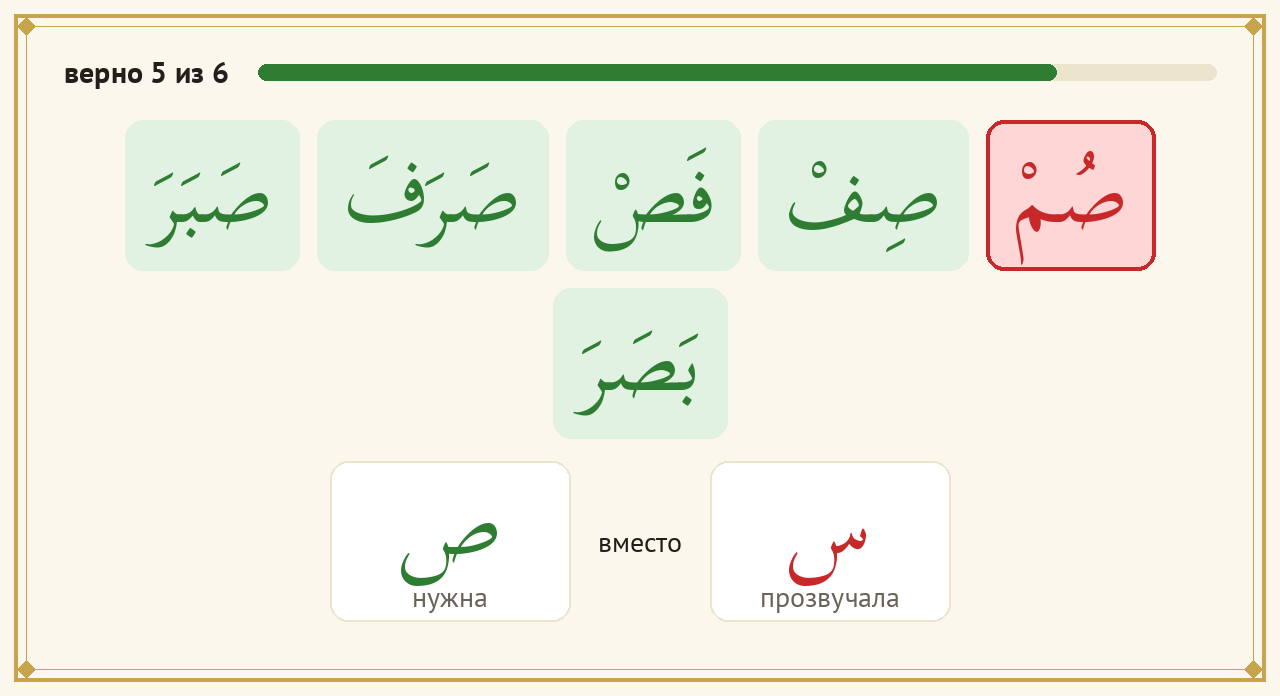
\includegraphics[width=0.78\linewidth]{screen-result.png}
  \caption{После попытки: слог с ошибкой подсвечен в строке.}
\end{subfigure}
\caption{Изображения карточек, которые строит тренажёр.}\label{fig:screens}
\end{figure}

\paragraph{Разбор ошибок} После попытки ученик видит строку с подсвеченными слогами
(рис.~\ref{fig:screens}б) и короткий разбор. Каждый пункт --- \emph{место}: слоги, задетые ошибкой, в виде
«как надо $\to$ как у тебя» транскрипцией, с подсказкой в полфразы. Явные ошибки (неверная буква или
огласовка) идут раньше ошибок долготы; перечисляется не больше трёх мест, остальные отмечены на картинке;
подробный совет по артикуляции свёрнут под «Подробнее»; разбор заканчивается одной строкой: послушай эталон
и прочитай строку ещё раз. Формат следует литературе об обратной связи из раздела~\ref{sec:lr-capt} и
заменил раннюю версию, где перечислялась каждая фонема и новички терялись. Хвалят за задачу («этот слог
теперь верно»), а не личность.

\paragraph{Транскрипция} Транскрипция русскими буквами помогает новичку, но может стать костылём. Как
компромисс между просьбой автора и советом преподавателей подсказка «Как читается» на карточке спрятана под
спойлер: сначала ученик пробует прочитать буквы. Транскрипция следует научной системе Крачковского в
упрощённом виде: точка снизу у эмфатических и горловых, черта снизу у межзубных, знаки для \emph{айна} и
хамзы --- так \ar{ص} и \ar{س} остаются различимыми \cite{SRC-051}.

\paragraph{Эталонное аудио} На каждой карточке со звуком есть кнопка «Послушать». Главнее всего запись
учителя, которую учитель может сделать прямо в боте. Иначе используются фрагменты обучающего чтения
аль-Хусари \cite{SRC-042}; каждый фрагмент проверяется моделью и выносится на проверку человеку до
использования. Синтез речи отклонён: он неверно передаёт таджвид.

\paragraph{Прочие функции} Кнопка «Бот ошибся» позволяет ученику оспорить вердикт с указанием причины;
оспоренные попытки идут в разметку первыми. Короткие вопросы на закрепление («как читается этот слог?»)
возвращают к пройденным буквам. На главном экране --- серия дней и число попыток за сегодня. Первый урок
начинается с \emph{истиазы} и \emph{басмалы}; таблица алфавита на с.~10 показывается для справки без проверки
голосом, потому что Максуди учит звукам, а не названиям.

\section{Исследовательские данные и разметка}\label{sec:impl-data}

\paragraph{Схема} Единица данных --- попытка. Ученики обозначены внутренним ID и псевдонимом; Telegram ID
хранится только в таблице учеников. Остальные таблицы содержат журнал согласий с версией текста согласия,
анкету при входе, снимок программы, найденные ошибки, разметку, разметчиков и приглашения, жалобы учеников
и журнал действий, в котором нет текстов сообщений. Одиннадцать SQL-отчётов и модуль метрик считают меры
GQM; попытки заглушки для разработки исключены везде.

\paragraph{Разметка} Разметчики работают в Telegram или с выгруженным пакетом (CSV-файл и аудио). В Telegram
доступ ограничен списком разметчиков или одноразовым кодом-приглашением, действующим сутки и отзываемым
сразу; права проверяются при каждом нажатии, записи отправляются так, что их нельзя переслать или
сохранить, и разметчик не видит, кто ученик. Загрузка строгая: одна неверная строка отклоняет файл,
повтор ничего не добавляет, исправленная метка добавляется с историей. Каждая метка хранит код
разметчика, версию руководства, источник и затраченное время.

\paragraph{Метрики и выгрузки} Модуль метрик считает TA/TR/FA/FR по фонемам, precision, recall, F1,
точность диагноза, FAR и FRR, $\kappa$ Коэна, $\alpha$ Криппендорфа (проверена на разобранном примере из
статьи Криппендорфа \cite{SRC-065}), процентили времени ответа, сбои распознавания и возвращаемость.
Наборы данных выгружаются только по согласившимся ученикам, под псевдонимами, с файлами \texttt{truth.csv}
и \texttt{predictions.csv} в формате Iqra'Eval, чтобы результаты можно было сравнить инструментами
соревнования \cite{SRC-066}.

\paragraph{Сохранность} Резервные копии содержат контрольные суммы и проверяются; восстановление сверяет
хеши, просит подтверждения и выполняется одной транзакцией. Команда сверки сравнивает базу с хранилищем
аудио и находит потерянные, лишние и повреждённые файлы, а также копии, которые должны были быть удалены
после отзыва согласия.

\section{Приватность и безопасность}\label{sec:impl-privacy}

\paragraph{Согласие и удаление} Сначала ученик видит экран согласия; согласие на запись голоса отдельное и
необязательное, кнопки не окрашены, чтобы не подталкивать, и тренажёр работает без него. Отзыв согласия
удаляет записи и разметку по ним; «Удалить мои данные» удаляет все строки и файлы ученика. В логах есть
псевдонимы и идентификаторы попыток, но нет Telegram ID, текстов сообщений, аудио и фонем; фильтр
вычищает секреты вроде токена бота; события согласия, удаления и разметки пишутся только в базу, не в
логи. Эти правила обеспечивают тесты.

\paragraph{Модель угроз} Анализ STRIDE охватывает подмену (личность --- только по подписанному Telegram ID;
нет входящих портов благодаря long polling), изменение (аудио адресуется по SHA-256; восстановление со
сверкой; замороженные тесты против подгонки), раскрытие (выгрузки под псевдонимами; агенту запрещено
читать данные учеников и секреты; файлы доступны только владельцу), отказ в обслуживании (ограничение
60 секунд) и повышение привилегий (параметризованные запросы, аудит зависимостей, контейнер не от root и
хук, блокирующий несуществующие пакеты).

\paragraph{Закрытый пилот и долг безопасности} Часть мер --- шифрование при хранении, выбор хостинга,
формальный статус оператора --- зависит от решений института. Чтобы не останавливать всю работу, проект
ведёт закрытый пилот и записывает каждую отложенную меру как пункт технического долга с явным
триггером: пункты «до чужих» должны быть закрыты прежде, чем будет приглашён кто-либо вне закрытого круга.

\section{Обвязка разработки}\label{sec:impl-harness}

Тренажёр создан одним автором вместе с Claude Code. Обвязка вокруг агента состоит из четырёх слоёв:
контекст (инструкции, решения и требования, которые агент должен знать), принуждение (хуки, которые
выполняет среда, а не модель), роли (субагенты с узкими задачами и ограниченными правами) и человек
(решения, которые нельзя делегировать). Цикл показан на рис.~\ref{fig:harness}.

\begin{figure}[ht]
\centering
\resizebox{\linewidth}{!}{% Обвязка ИИ-агента (agent harness): направляющие, датчики, человек (ADR-0011, ADR-0012, ADR-0034, ADR-0039).
% Рамка guides/sensors — SRC-029.
\begin{tikzpicture}[node distance=5mm and 8mm]
  \node[goldbox,text width=3.3cm,xshift=-4mm] (guides) {\textbf{\LANG{Guides}{Направляющие}}\\[-1pt]{\scriptsize CLAUDE.md, ADR, \LANG{skills, requirements}{скиллы, требования}}};
  \node[hot,right=of guides,text width=3.0cm] (agent) {\textbf{\LANG{Coding agent}{ИИ-агент}}\\[-1pt]{\scriptsize\LANG{reason $\to$ act $\to$ observe}{рассуждение $\to$ действие $\to$ наблюдение}}};
  \node[box,right=of agent,text width=3.6cm] (pre) {\textbf{PreToolUse}\\[-1pt]{\scriptsize guard, human\_zones, dep\_check, git\_guard}};
  \node[box,below=of pre,text width=3.6cm] (act) {\LANG{Edit / run}{Правка / команда}\\[-1pt]{\scriptsize\LANG{tests frozen in \texttt{impl}}{тесты заморожены в \texttt{impl}}}};
  \node[box,below=of act,text width=3.6cm] (stop) {\textbf{Stop gate}\\[-1pt]{\scriptsize import-linter, mypy --strict, pytest}};
  \node[box,left=13mm of stop,text width=3.0cm] (rev) {\LANG{Reviewer subagents}{Субагенты-ревьюеры}\\[-1pt]{\scriptsize\LANG{code, architecture, direction}{код, архитектура, направление}}};
  \node[human,left=15mm of rev,text width=3.3cm] (human) {\textbf{\LANG{Human}{Человек}}\\[-1pt]{\scriptsize\LANG{accepts tests, content, commits}{принимает тесты, контент, коммиты}}};
  \node[store,below=8mm of rev,text width=4.2cm,minimum height=1cm] (log) {\LANG{Journals}{Журналы}\\[-1pt]{\scriptsize\LANG{prompts, hook blocks, sessions}{запросы, блокировки, сессии}}};

  \draw[arr] (guides) -- (agent);
  \draw[arr] (agent) -- (pre);
  \draw[arr] (pre) -- node[lab,right]{\LANG{allowed}{разрешено}} (act);
  \draw[arr,draw=lesson] (pre.north) -- ++(0,5mm) -| node[lab,text=lesson,above,pos=0.25]{\LANG{blocked, with reason}{блок с причиной}} (agent.north);
  \draw[arr] (act) -- (stop);
  \draw[arr,draw=lesson] (stop.east) -- ++(5mm,0) |- node[lab,text=lesson,right,pos=0.25]{\LANG{red: keep working}{красно: продолжать}} (act.east);
  \draw[arr] (stop) -- node[lab,above]{\LANG{green}{зелено}} (rev);
  \draw[arr] (rev) -- node[lab,above]{\LANG{STOP $\to$ ask}{СТОП $\to$ вопрос}} (human);
  \draw[arr] (human) -- (guides);
  \draw[darr] (stop.south) |- (log.east);
  \draw[darr] (rev) -- (log);
  \node[lab,above=1mm of guides] {\LANG{feed-forward}{до действия}};
  \node[lab,above=7mm of pre] {\LANG{feedback (sensors)}{после действия (датчики)}};
\end{tikzpicture}
}
\caption{Обвязка агента: направляющие, датчики и человек (ср.\ Р-06).}\label{fig:harness}
\end{figure}

\paragraph{Хуки} Одиннадцать хуков перечислены в таблице~\ref{tab:hooks}. Хук guard работает по принципу
fail-closed: если он сам упал, действие запрещается.

\begin{table}[ht]
\centering\small
\caption{Хуки обвязки.}
\label{tab:hooks}
\begin{tabularx}{\linewidth}{@{}P{3.0cm}P{2.6cm}L@{}}
\toprule
Хук & Событие & Что делает \\
\midrule
guard & до вызова инструмента & Запрещает чтение секретов и данных учеников, правку тестов в фазе
реализации, прямую смену фазы, обход проверок, force push. \\
human\_zones & до вызова инструмента & Требует подтверждения с причиной перед изменением контента, текстов
ученику, порогов, параметров чтения, схемы, зависимостей, самих проверок и оценщика RQ-1. \\
dep\_check & до вызова инструмента & Блокирует пакеты, которых нет на PyPI; для остальных показывает
версию, возраст, репозиторий, известные уязвимости и похожесть имени. \\
git\_guard & до вызова инструмента & Запрещает принудительное добавление, запрещённые пути и секреты в
коммитах; push --- только при зелёных проверках. \\
format\_python & после вызова инструмента & Форматирует и проверяет изменённые файлы, возвращает
оставшиеся замечания. \\
stub\_notice & после вызова инструмента & Напоминает агенту сказать человеку, что бот запущен с
заглушкой распознавания. \\
stop\_gate & завершение & Агент не может закончить, пока не проходят контракты слоёв, типы или тесты. \\
doc\_sync & завершение & «Изменил X --- обнови Y»: журнал изменений, словарь данных, отчёты, схемы,
версии текстов согласия, трассировка. \\
log\_prompt & запрос & Сохраняет каждый запрос человека с датой (секреты маскируются). \\
session\_context & начало сессии & Загружает TDD-фазу, состояние модели, открытый блокирующий долг и
сводку прошлой сессии. \\
notify & уведомление & Системное уведомление, когда агент ждёт человека. \\
\bottomrule
\end{tabularx}
\end{table}

\paragraph{Фазы TDD} Изменение проходит явные фазы. В фазе \emph{тестов} субагент пишет падающие тесты, а
аудитор тестов проверяет, что они способны ловить ошибки; автор принимает тесты. В фазе \emph{реализации}
тесты заморожены хуком guard, и исполнитель пишет код, пока все проверки не пройдут. Изменение принятого
теста требует возврата в фазу тестов с согласия автора; журналы фиксируют каждый такой случай.

\paragraph{Субагенты} Двадцать один субагент имеет узкую роль. Пишущие (автор тестов, исполнитель,
летописец диссертации) могут менять только свои области; проверяющие (ревьюер кода, страж архитектуры,
аудитор безопасности, аудитор тестов, аудитор согласованности, ревьюер направления) права записи не имеют.
Ревьюер направления проверяет, делает ли изменение то, о чём просил автор, и остаётся ли в полномочиях
агента; при сомнении он обязан вернуть СТОП с вопросами автору, а не догадку. «Водитель бота» проходит
настоящие обработчики в консольном режиме без Telegram, секретов и базы учеников, а «симулятор ученика»
читает интерфейс глазами новичка --- с оговоркой, что симулированные ученики не настоящие \cite{SRC-083}.

\paragraph{Решения и журналы} Когда есть выбор, агент должен показать два--четыре варианта с плюсами и
минусами, а не выбирать молча; выбранный и отклонённые варианты записываются в ADR. Записано пятьдесят
ADR, включая отклонённые идеи вроде Redis, вебхуков, Mini App и синтеза речи. Каждая сессия заканчивается
сводкой просьб, решений, отклонений и непроверенного. Коммиты готовит отдельная команда, которая
запускает проверки, сверяет документацию и просит автора подтвердить каждый коммит и push.

\section{Проверка качества}\label{sec:impl-verification}

Набор тестов выполняется меньше чем за минуту без модели и сети и сейчас содержит 736 проходящих тестов.
В нём модульные тесты домена, интеграционные тесты репозиториев на SQLite (и PostgreSQL в CI), сквозные
тесты сценария бота через диспетчер, архитектурные тесты (контракты слоёв, соответствие миграций схеме,
регистрация каждого сценария, отсутствие запрещённых полей в логах, ссылки документов на существующие
файлы) и тесты свойств, которые должны выполняться для любого эталона и любого выхода модели: чтение
точно по эталону даёт идеальный результат; балл лежит в пределах 0--100, и каждая ошибка указывает внутрь
эталона; оценка детерминирована; «отлично» ставится только без ошибок; недочитанный хвост указывает на
существующий слог; лучший эталон --- ближайший, при равенстве --- первый \cite{SRC-096}. Обычный прогон
проверяет 300 случайных примеров на свойство; разовый прогон с 5\,000 примеров на свойство нарушений не
нашёл. Покрытие строк выше 97\,\% при минимуме 80\,\% в CI; mypy работает в строгом режиме. Непрерывная
интеграция добавляет поиск секретов, аудит уязвимостей зависимостей, проверку объявленных зависимостей,
статическую проверку самих workflow и сборку Docker-образа. Автоматический отчёт трассировки показывает,
что 59 из 60 прослеженных требований покрыты проходящими тестами.
